%% The following is a directive for TeXShop to indicate the main file
%%!TEX root = diss.tex

\chapter{Related Work}
\label{ch:RelatedWork}
Section~\ref{sec:Toolbox} discusses the existing toolboxes for 3D reconstruction. Section~\ref{sec:3DRecon_Tech} presents a comprehensive review of the field of image-based 3D reconstruction based on varied visual/geometri cues, which include \textit{stereo correspondence}, \textit{shading}, \textit{silhouette}, \textit{texture distortion}, and \textit{(de)focus}.

\section{ToolBoxes}
\label{sec:Toolbox}
There have been many attempts in developing computer vision or image processing frameworks that support rapid development of vision applications. There are multiple general vision libraries in the field including OpenCV~\cite{bradski2008learning}, VLFeat~\cite{vedaldi08vlfeat}, [VXL]~\cite{vxl17} and multiple Matlab libraries~\cite{KovesiMATLABCode, MariottiniPr_RAM05}. These libraries often provide tools to multiple image processing and computer vision problems, including low-vision tasks such as feature detection and matching, middle-level vision tasks such as segmentation, tracking, and high-level vision problems such as classification and recognition. All of these software frameworks and libraries provide vision components and algorithms without any context of how and when they should be applied, and so often require expert vision knowledge for effective use.

\section{3D Reconstruction Techniques}
\label{sec:3DRecon_Tech}
Image-based 3D reconstruction attempts to recover the geometry and optionally the material of the object from images under different viewpoints or illuminations. The goal can be described as ``given a set of images of an object or a scene, estimate the most likely 3D shape that explains those images, under the assumption of known materials, viewpoints, and lighting conditions''. This definition reveals that if those assumptions are invaild, this becomes an ill-posed problem since multiple combinations of geometry, viewpoint and illumination can produce exactly the same images~\cite{poggio1985computational}, thus making it an extremely challenging task.

The 3D reconstruction techniques exploits a variety of visual and geometric cues to extract geomtry from images: stereo correspondence, shading, contour, texture, (de)focus, etc. Refer to Table~\ref{tab:cue_algo} for the cue used by each class of algorithms. The algorithms are organized based on the cue used for reconstruction in this review.
\begin{table}[h]
  \centering
  \begin{tabular}{l|r}
  \hline
  \textbf{Cue} & \textbf{Algorithm}\\
  \hline\hline
  Stereo correspondence & Stereoscopy\\
  & Trinocular Stereo\\
  & Multi-view Stereo (MVS)\\
  & Laser scanning\\
  & Structured light (SL)\\
  \hline
  Shading & Shape from Shading (SfS)\\
  & Photometric Stereo (PS)\\
  \hline
  Contour & Shape from Silhouette (SfS)\\
  \hline
  Texture & Shape from Texture\\
  \hline
  (De)focus & Shape from (De)focus\\
  \hline
  \end{tabular}
  \caption{Classes of algorithms that utilize each visual/geometric cue. Note that the abbreviations will be used extensively in the theis, and the actuall meaning of SfS can be deduced from the context.}
  \label{tab:cue_algo}
\end{table}

\subsection{Stereo Correspondence}
Stereo correspondence is one of the most widely used visual cues in 3D vision. Passive methods, including stereoscopy, trinocular stereo, and MVS, identify correspondences across different views, and estimate the 3D point by triangulation. However these passive approaches suffer from uniform or periodic surfaces. The active techniques attempt to overcome the correspondence problem by replacing one of the cameras with a controllable illumination source, e.g., single-point laser, slit laser scanner, and temporal or spatially modulated Structured Light (SL), we refer the readers to the survey article by \citeauthor{blais2004review} for recent development of active methods. Two most popular methods, MVS and SL, are reviewed in depth, and organized based on the reconstruction algorithms and projection patterns used, respectively.

\subsubsection{Volumetric methods}
The first class computes the cost function in a 3D volume, then extracts a surface from this volume. One successful algorithm is voxel colouring, which traverses a discretized 3D space in “depth-order” to identify voxels that have a unique colouring, constant across all possible interpretations of the scene~\cite{seitz1997photorealistic}. Another thread of work formulates the problem in the Markov Random Field (MRF) framework and extracts the optimal surface by Graph-Cut algorithms~\cite{roy1998maximum,vogiatzis2005multi,vogiatzis2007multiview}.

\subsubsection{Surface Evolution}
The second class works by iteratively evolving a volume or surface to minimize a cost function. The class includes methods based on voxels, level set, and surface meshes. Space Carving technique achieves least-commitment shape \cite{marr1982vision} by iteratively removing inconsistent voxels from the scene~\cite{kutulakos2000theory}. Level-set techniques cast the problem as a variational one, and use a set of PDE's as cost functions, which are deformed from an initial set of surfaces towards the objects to be detected~\cite{faugeras2002variational}. Other approaches use a deformable model and represent the scene as surface meshes that moves as a function of internal and external forces~\cite{esteban2004silhouette}. \citeauthor{hiep2009towards} presented a visibility-based method that transforms a dense point cloud into a surface mesh, which is feed into a mesh-based variational refinement that captures small details, smartly handling photo-consistency, regularization and adaptive resolution.

% Level-set based techniques minimize a set of partial differential equations defined in a volume. Like space carving methods, level-set methods typically start from a initial volume and shrink inward, or outward if the cost function is minimized. \citeauthor{faugeras2002variational} proposed a novel geometric approach based on variational principle, from which a set of PDE's can be deduced. The level set method is used to deform an initial set of surfaces towards the objects to be detected. However, level-set is no long a popular MVS technique, because high quailty models with correct topology can be directly computed from photo-consistency functions without the refinement steps.

\subsubsection{Region Growing}
The third class starts with a sparse set of scene points, and propagates these points to spatial neighbours and refine the cost function with respect to position and orientation of the points. \citeauthor{otto1989region} proposed one of the first work on region growing stereo search. The essence of the algorithm is: start with an approximate match between a point in one image and a point in another, use an adaptive least-squares correlation algorithm to produce a more accurate match, and use this to predict approximate matches for points in the neighbourhood of the first match. A two-view quasi-dense approach first sorts the list of point correspondences into a list of seed points by correlation score. At each step of the propagation, A `best' seed point is chosen. Then in the immediate spatial neighborhood of this seed point, new potential matches are checked and the bests are added to the current list of seed points~\cite{lhuillier2002match,lhuillier2005quasi}. This best-first strategy guarantees convergence by choosing only new matches that have not yet been selected. A patch based approach undergoes multiple iterations of matching, propagation, and filtering~\cite{furukawa2010accurate}. A stereoscopic approach called PatchMatch Stereo, which is inspired by an approximate nearest neighbour matching algorithm called PatchMatch~\cite{Barnes:2009:PAR}. The method starts by randomly assigning an oriented plane to each pixel in two views. Then each pixel goes through three iterations of propagations and refinement. The plane is propagated to spatial neighbours, corresponding pixel from another view, and across time. It can achieve sub-pixel accuracy, but is computational heavy and difficult to parallelism. There has been some efforts to extend PatchMatch Stereo to multi-view scenario~\cite{galliani2015massively,uh2014efficient,zheng2014patchmatch} or proposing new propagation scheme to increase the computational efficiency~\cite{galliani2015massively}.
%[has nice math derivations] Shen, Accurate Multiple View 3D Reconstruction Using Patch-Based Stereo for Large-Scale Scenes\\

\subsubsection{Depthmap Merging}
The fourth class is image-space based methods that computes a per-view depthmap. By treating a depthmap as a 2D array of 3D points, multiple depthmaps can be considered as a merged 3D point cloud. The winner-takes-all approach takes a set of discretised depth values and pick the one with the highest photo-consistency score for each pixel independently. Uniform depth sampling may suffice for simple and compact objects. However, for complex and large scenes, a proper sampling scheme is crucial to achieve high speed and quality. More sophisticated cost function are derived to account for occlusion or non-Lambertian effects which might add noise to the photo-consistency score~\cite{goesele2006multi,vogiatzis2007multiview}. In the case of severe occlusion, spatial consistency can be enforced under the assumption that neighbouring pixels have similar depth values. This can be formulated under the Markov Random Field (MRF) framework, where the problem becomes minimizing the sum of a unary $\Phi(\cdot)$ and pairwise term $\Psi(\cdot, \cdot)$. The unary term reflects the photo-consistency score of assigning a depth value $d_p$ from a depth set to the pixel $p$, whereas the pairwise term enforces the spatial regularization, and assigns the cost of setting depth label $k_p$, $k_q$ to a pair of neighbouring pixels $p$ and $q$, respectively.
$$
E(\{k_p\})= \sum_p \Phi(k_p) + \sum_{(p,q)\in\mathcal{N}}\Psi(k_p, k_q)
$$

\subsubsection{Structured Light}
Structured light is considered one of the most accurate reconstruction technique. It is based on projecting a temporally or spatially modulated pattern onto the surface and viewing the illuminated surface from one or more points of view. The correspondence is easily detected from the projected and imaged pattern, which is triangulated to obtain the 3D point. Each pixel in the pattern is assigned a unique codeword, and the codeword is encoded by using grey level, colour or geometric representations. Structured light is classified based on the coding strategy: temporal, spatial and direct codification \cite{salvi2004pattern}. Temporal techniques generate the codeword by projecting a sequence of patterns. Spatial codification represents each codeword in a unique pattern. Direct codification techniques define a codeword for every pixel, which is equal to its grey level or colour.

\textbf{Temporal encoding} A sequence of patterns are successively projected onto the surface, the codeword for a given pixel is formed by the sequence of illuminaiton values for that pixel across the projected patterns. This kind of pattern can achieve high accuracy due to two factors: 1). the codeword basis is small, e.g., two for binary pattern, therefore, each bit is easily distinguishable; 2). a coarse-to-fine strategy is used, and the position of the pixel becomes more precise as the patterns are successively projected. We further classify these techniques as follows: 1). binary codeword; 2). $n$-ary codeword; 3). gray code combined with phase shifting; 4). hybrid techniques.

\textbf{Spatial encoding} This kind of technique concentrate all the coding in a unique pattern. The codeword that labels a certain pixel is obtained from a neighbourhood of the pixels around it. Normally, the visual features gathered in a neighbourhood are the intensity or colour of the pixels or groups of pixels around it.

\textbf{Direct encoding} There are ways that can directly represent the codeword in each pixel. To achieve this, there is a need to use either a large range of colour values or introduce periodicity. However, this kind of pattern is highly sensitive to noise because the ``distance'' between codewords is nearly zero. Moreover, the perceived colour depends not only on the projected colour, but also the intrisic clour of the surface, therefore, reference images must be taken. This kind of coding can be classified as: 1). codification based on grey levels; 2). codification based on colour.

\subsection{Shading}
The shading variations can reveal the surface normal orientation, which can be further integrated into a 2.5D height map. Shading variation depends on the shape (surface normal orientation), reflectance (material), and lighting (illumination), therefore is generally a ill-posed problem because difference shapes illuminated under different light conditions might produce the same image. This leads to a novel technique called Photometric Stereo in which surface orientaiton is determined from two or more images. The idea of Photometric Stereo is to vary the direction of the incident illumination between successive views while holding the viewing direction constant. This provides enough information to determine surface orientation at each pixel~\cite{woodham1979photometric}. This technique can produce a surface normal map with the same resolution of the input image, \ie to produce the pixel-wise surface normal map. Since the coefficients of the normal are continous, the integrated height map can reach an accuracy that cannot be achieve by any triangulation methods. Therefore, photometric stereo is more desirable if the intrisic geometric details are of great importance.

\subsubsection{Shape from Shading}
The problem of recovering the shape of a surface from the intensity variation is first proposed by Horn~\cite{horn1970shape}. It assumes that the surface under consideration is of a uniform albedo and reflectance, and that the direction of the single distant light source is either known or can be calibrated by the use of a reference object. Thus the intensity $I(x,y)$ becomes purely a function of the local surface orientation. The information of reflectance, illumination, and viewing geometry can be combined into a single function called reflectance map $R(p, q)$, that relates surface orientation directly to image intensities
\begin{align*}
I(x, y) &= R(p(x, y), q(x, y))\\
I(x, y) &= \rho(\vec{n},\vec{l})\vec{n}^\top\vec{l} \quad (\text{Lambertian model})
\end{align*}
where $(p, q) = (z_x, z_y)$ are surface gradients. Unfortunately, measurements of the brightness at a single pixel only provide one constraint whereas surface orientation requires two. Thus additional constraints such as smoothness or integrability is required to estimate $(p, q)$.

\subsubsection{Photometric Stereo}
\begin{table}[h]
  \centering
  \begin{tabular}{l|*{4}{c}}
  \hline
  \textbf{Category} & Camera & Light source & Reflectance & Others\\
  \hline
  Original PS & Orthographic & Directional, known intensity and direction & Lambertian & No shadow, interreflection.\\
  Generalized lighting PS & Orthographic & unknown intensity and direction, ambient & Lambertian & \\
  Generalized reflectance PS & Orthographic & Distant, known intensity and direction & Non-Lambertian & \\
  \hline
  \end{tabular}
  \caption{Assumptions made by different classes of photometric stereo.}
  \label{tab:ps_assumptions}
\end{table}

\textbf{Original Photometric Stereo} This method, first proposed by Woodham~\cite{woodham1980photometric}, utilised multiple light sources from different directions to overcome the ambiguity of Shape from Shading. Assume there are $P$ pixels per image, and $Q$ illumination directions, the intensity of the $i$th pixel under $j$th illumination would be
\begin{align*}
I_{i,j} &= \rho_i\vec{n}_i^\top \vec{l}_j\\
\Rightarrow\mathbf{I} &= \mathbf{N}^\top \mathbf{L}
\end{align*}
where
\begin{itemize}
\item $\mathbf{I}\in \mathbb{R}^{P\times Q} $stores the pixel intensity from all images. Each column contains pixels from each image while each rows contains intensity of each pixel under all illumination conditions
\item $\mathbf{N}\in \mathbb{R}^{P\times3}$ encodes the albedo-scaled surface normal for each pixel, \ie $N_{i, :} = \rho_i\vec{n}_i^\top$
\item $\mathbf{L} \in \mathbb{R}^{3\times Q}$ encodes the light source directions, \ie $L_{:, j} = \vec{l_j}$
\end{itemize}
This surface reflectance, \ie spatially varying albedo, and the normal can be estimated by
\begin{align*}
N &= IL^{+}\\
\rho_i &= \|N_{i,:}\|\\
n_i &= \frac{N_{i,:}^\top}{\|N_{i,:}\|}
\end{align*}

The key problem is how to generalize the assumptions of photometric stereo. For the camera assumption, orthographic projection can be achieved by using a lens with long focus and placing the objects far from the camera. The nonlinear response can be solved by performing radiometric calibration. The shadow and other global light transportation are one of the sources of errors, some approaches consider them as outliers and remove them before normal estimation. The reflectance and lighting assumptions, however, are the most complicated ones since the reflectance properties depends on material property and the microscopic structure, and the lighting can have arbitray or fixed position, orientation, and intensity. Therefore the research on Photometric Stereo are generally on two directions: 1). generalization of reflectance; 2). generalization of lighting conditions.

\textbf{Generalization of Lighting} It is possible to estimate the surface orientation without knowing the light directions, a case also known as \textit{uncalibrated Photometric Stereo}, see Table~\ref{tab:ps_assumptions}. Most such techniques assume Lambertian techniques and are based on factorization technique proposed in \cite{hayakawa1994photometric}. Recall the Irradiance equation:
$$
I=N^\top L
$$
However, an infinite number of candidates $\hat{N}$ and $\hat{L}$ make the above equality met. In fact, any invertible $3\times 3$ matrix $G$ defines a candidate pair $\hat{N} = N\cdot G, \hat{L}=G^{-1}L$. Thus the normal $N$ and light source direction $L$ can only be recovered up to a linear transformation.

Other generalized lighting conditions are anything other than the the ideal case of using a single distant point light source in a dark room. Therefore, any general cases like natural ambient light, multiple point light sources with/without ambient lighting, etc. To make the problem more tractable, the reflectance model should no longer be a general one, otherwise, the problem would have too many degrees of freedom, which means many different shapes with an incorrectly estimated general reflectance, and an incorrectly estimated general lighting would generate the same image appearance with much higher probability.

\textbf{Generalization of Reflectance} This class of techniques relax the assumption of Lambertian reflectance.

\textit{Outlier rejection} 
The fact that the reflectance of non-Lambertian surfaces can be approximated by the sum of a diffuse and a specular lobe has been exploited extensively. The specular pixels are considered as outliers in ~\cite{coleman1982obtaining} and \cite{barsky20034}. The assumption that the color of the specular lobe differs from that of the diffuse lobe allows the separation of the specular and diffuse components~\cite{mallick2005beyond,sato1994temporal,schluns1993photometric}.

\textit{Reference object}
A different approach uses a reference object that has the same material as the target object. This is proposed in~\cite{silver1980determining} and later revisited in~\cite{hertzmann2005example}. It can deal with arbitrary BRDFs as long as the reference and target object has the same material. Multiple reference objects are needed for spatially-varying BRDFs as the BRDF at each point on the target object is a linear combination of the basis BRDFs defined by the set of reference objects. 

\textit{Parametric reflectance model} 
More sophisticated BRDF models can replace the reference objects. An isotropic Ward model is used as basis BRDF, and the surface orientation and parameters of the reflectance models are estimated iteratively~\cite{goldman2010shape}.

\textit{Invariants of BRDF} 
While parametric reflectance models are very good at reducing the complexity of BRDFs, they are usually only vaid for a limited class of materials. An alternative is to exploit the invariants of BRDFs. Typical ones include energy conservation, non-negativity, Helmholtz reciprocity, isotropy, etc~\cite{zickler2002helmholtz,alldrin2007toward}.

% [Some other papers to read] \\
% - R. J. Woodham. Photometric method for determining sur-
% face orientation from multiple images.\\
% 1. joint recovery of unknown shape and reflectance\\
% - N. Alldrin, T. Zickler, and D. Kriegman. Photometric stereo with non-parametric and spatially-varying reflectance.\\
% - D. Goldman, B. Curless, A. Hertzmann, and S. Seitz. Shape and spatially-varying BRDFs from photometric stereo.\\
% - T. Higo, Y. Matsushita, and K. Ikeuchi. Consensus photometric stereo.\\
% - B.Shi,P.Tan,Y.Matsushita,and K.Ikeuchi. Elevationangle from reflectance monotonicity: Photometric stereo for general isotropic reflectances.\\
% - BOXIN SHI's PhD thesis\\
% - Satoshi Ikehata's PhD thesis\\
% 2. a less restrained capture setup with arbitrary and unknown illumination\\
% - H. Hayakawa. Photometric stereo under a light source with arbitrary motion\\
% - T. Papadhimitri and P. Favaro. A new perspective on uncalibrated photometric stereo\\
% - B. Shi, Y. Matsushita, Y. Wei, C. Xu, and P. Tan. Self-calibrating photometric stereo\\
% 3. combine both directions\\
% - A.Hertzmannand S.Seitz.Shapeandmaterialsbyexample: a photometric stereo approach.\\
% - A. Hertzmann and S. Seitz. Example-based photometric stereo: shape reconstruction with general, varying BRDFs.\\
% - W. M. Silver. Determining shape and reflectance using mul- tiple images. Master’s thesis, MIT, 1980.\\

\subsection{Silhouette}
In some cases, it's an easy task to perform a foreground segmentation of the object of interest, which leads to a class of techniques that reconstructs a 3D volumetric model from the intersection of the binary silhouettes projected into 3D. The resulting model is called a \textit{visual hull}.

The basic idea of shape from silhouette algorithms is that the object lies inside the intersection of all visual cones back-projected from silhouettes. Suppose there are multiple views $V$ of the target object. From each viewpoint $v\in V$, the silhouette $s_v$ can be extracted, which is the region including the object's interior pixels and delimited by the line(s) separating the object from the background. The silhouette $s_v$ are generally non-convex and can represent holes due to the geometry of the object. A cone-like volume $cone_v$ called (truncated) extended silhouette is generated by all the rays starting at the center of projection and passing through all the points of the silhouette. The target object is definitely internal to $cone_v$ and this is true fro every view $v'\in V$; it follows that the object is contained inside the volume $c_V=\cap_{v\in V}c_v$. As the size of the $V$ goes to infinity, and all possible views are included, $c_V$ converges to a shape known as the \textit{visual hull} $vh$ of the target object.

% Some approaches first approximate each silhouette with a polygonal representation and then intersect the resulting faceted conical regions in 3D space to produce polyhedral models, which can be later refined using triangular splines. Other approaches use voxel-based representations, usually encoded as octrees, because of the resulting time-space efficiency.

[computational complexity] intersection of many volumes can be slow. Simple polyhedron-polyhedron intersection algorithms are inefficient. To improve performance, most methods 1) quantize volumes, 2) perform intersection computation in 2D instead of 3D.

\subsubsection{Voxel based methods}
First the object space is split up into a 3D grid of voxels; each voxel is intersected with each silhouette volume; only voxels that lie inside all silhouette volumes remain part of the final shape.

\subsubsection{Marching intersections based methods}
The marching intersection (MI) structure consists of 3 orthogonal sets of rays, parallel to the $X$, $Y$, and $Z$ axis, which are arranged in 2D regular arrays, called the $X-rayset$, $Y-rayset$, $Z-rayset$ respectively. Each ray in each rayset is projected to the image plane to find the intersections with the silhouette. These intersections are un-projected to compute the 3D intersection between the ray and the extended silhouette on this ray. This process is repeated for each silhouette, and the un-projected intersections on the same ray are merged by the boolean AND operation.

Once the MI data structure representing the intersection of all extended silhouettes, a triangular mesh is extrated from it. This is done by the MI technique proposed in~\cite{rocchini2001marching} which traverses the ``virtual cells'' implicitly defined by the MI, builds a proper marching cube (MC) entry for them that in turn is used to index a MC's lookup table.
\begin{figure}[h]
\centering
\begin{tabular}{cc}
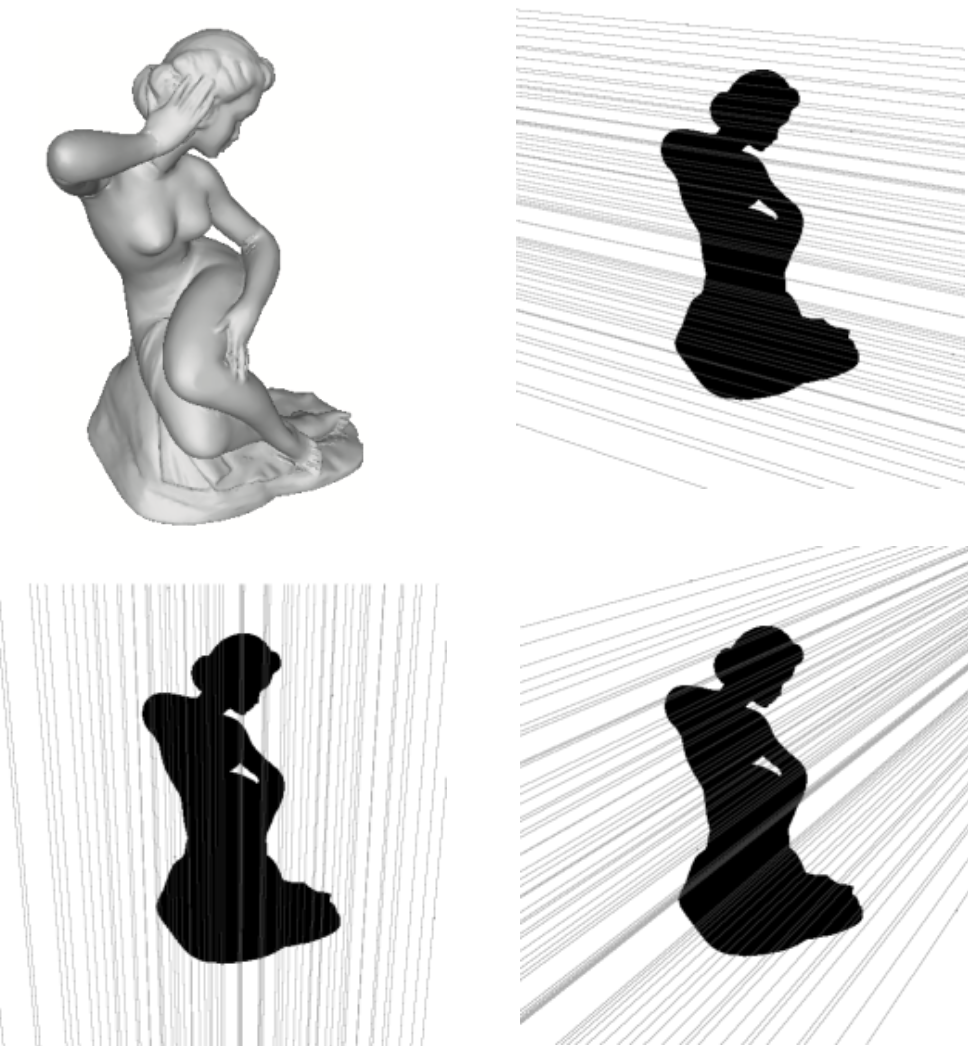
\includegraphics[width=0.5\textwidth]{relatedwork/scan_convert}&
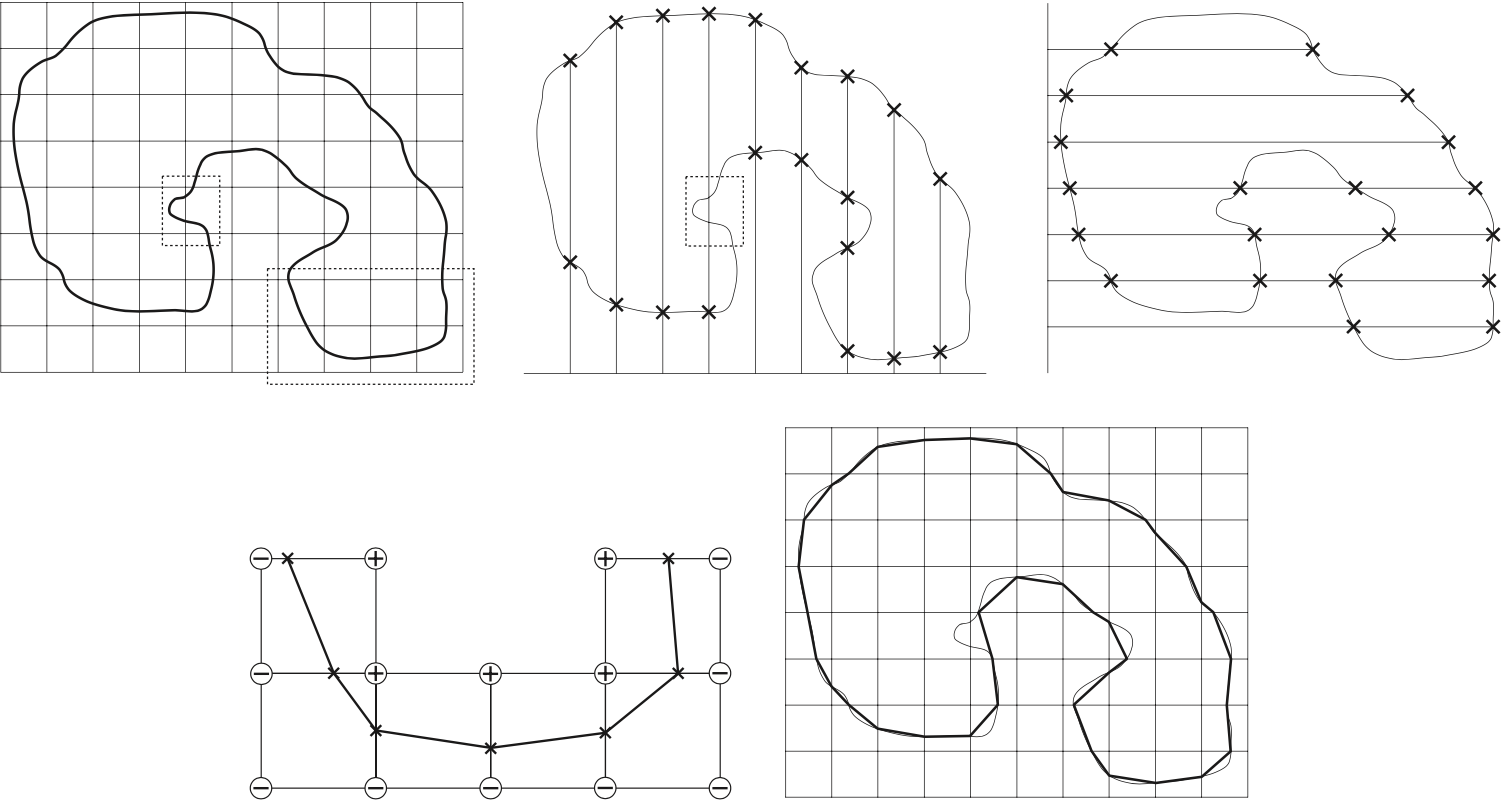
\includegraphics[width=0.5\textwidth]{relatedwork/mi_struct}\\
(a) & (b)\\
\end{tabular}
\caption{Illustratives of MI-based VH. (a) shows one object (top left) and its silhouette with 2D lines traced over it to find intersections along rays in the X, Y and Z ray-set of the MI, respectively. (b) shows the MI data structure and conversion algorithm in a 2D example. Image courtesy of M. Tarini.}
\label{fig:robust_pc}
\end{figure}

\subsubsection{Exact polyhedral methods}
The silhouette is converted into a set of convex or non-convex 2D polygons with holes allowed. The resulting visual hull with respect to those polygonal silouettes is a polyhedron. The faces of this polyhedron lie on the faces of the original cones. The faces of the original cones are defined by the center of projections and the edges in the input silhouettes. The idea of this method is: for each input silhouette $s_i$ we compute the face of the cone. Then we intersect this face with cones of all other input silhouettes, \ie a polygon-polyhedron intersection. The result of these intersections is a set of polygons that define the surface of the visual hull.

% \subsection{Image based method}
% \begin{itemize}
% \item this algorithm will only produce renderings of a visual hull from any view
% \item every pixel in the desired output image is back-projected to form a 3D ray
% \item each of those rays is intersected with each of the input silhouettes in the same way as the rays in the marching intersections method
% \item a pixel in the output image is inside the new rendering of the visual hull if its ray has any segments left in it that are intersecting the visual hull. The depth of these pixels is known from the depth of the nearest entry point on the ray.
% \end{itemize}

All of the cues above are most widely used ones, and achieved decent results. These following two cues haven't resulted in as much success. Therefore, we only discuss the general idea rather than the technical details.

\subsection{Texture}
The basic principle behind shape from texture is the \textit{distortion} of the individual texel. In general, the image formation process introduces three distortion effects: the \textit{distance effect}, which makes objects in view appear larger when they are closer to the image plane; the \textit{position effect} which makes objects appear differently when the angle between the line of sight and the image plane different; and the \textit{forshortening effect}, which distort the objects depending on the angle between the surface normal and the line of sight. Besides, different effects take place under different projection models: the orthographic projection captures only the foreshortending effect whereas the perspective projection captures all three. Therefore, shape from texture methods which use orthographic projection are valid only in a limited domain, where the other two effects can be ignored, and the perspective model captures all three effects, but the resulting algorithms are complicated and involves the solution of nonlinear equations.
\begin{figure}[h]
\centering
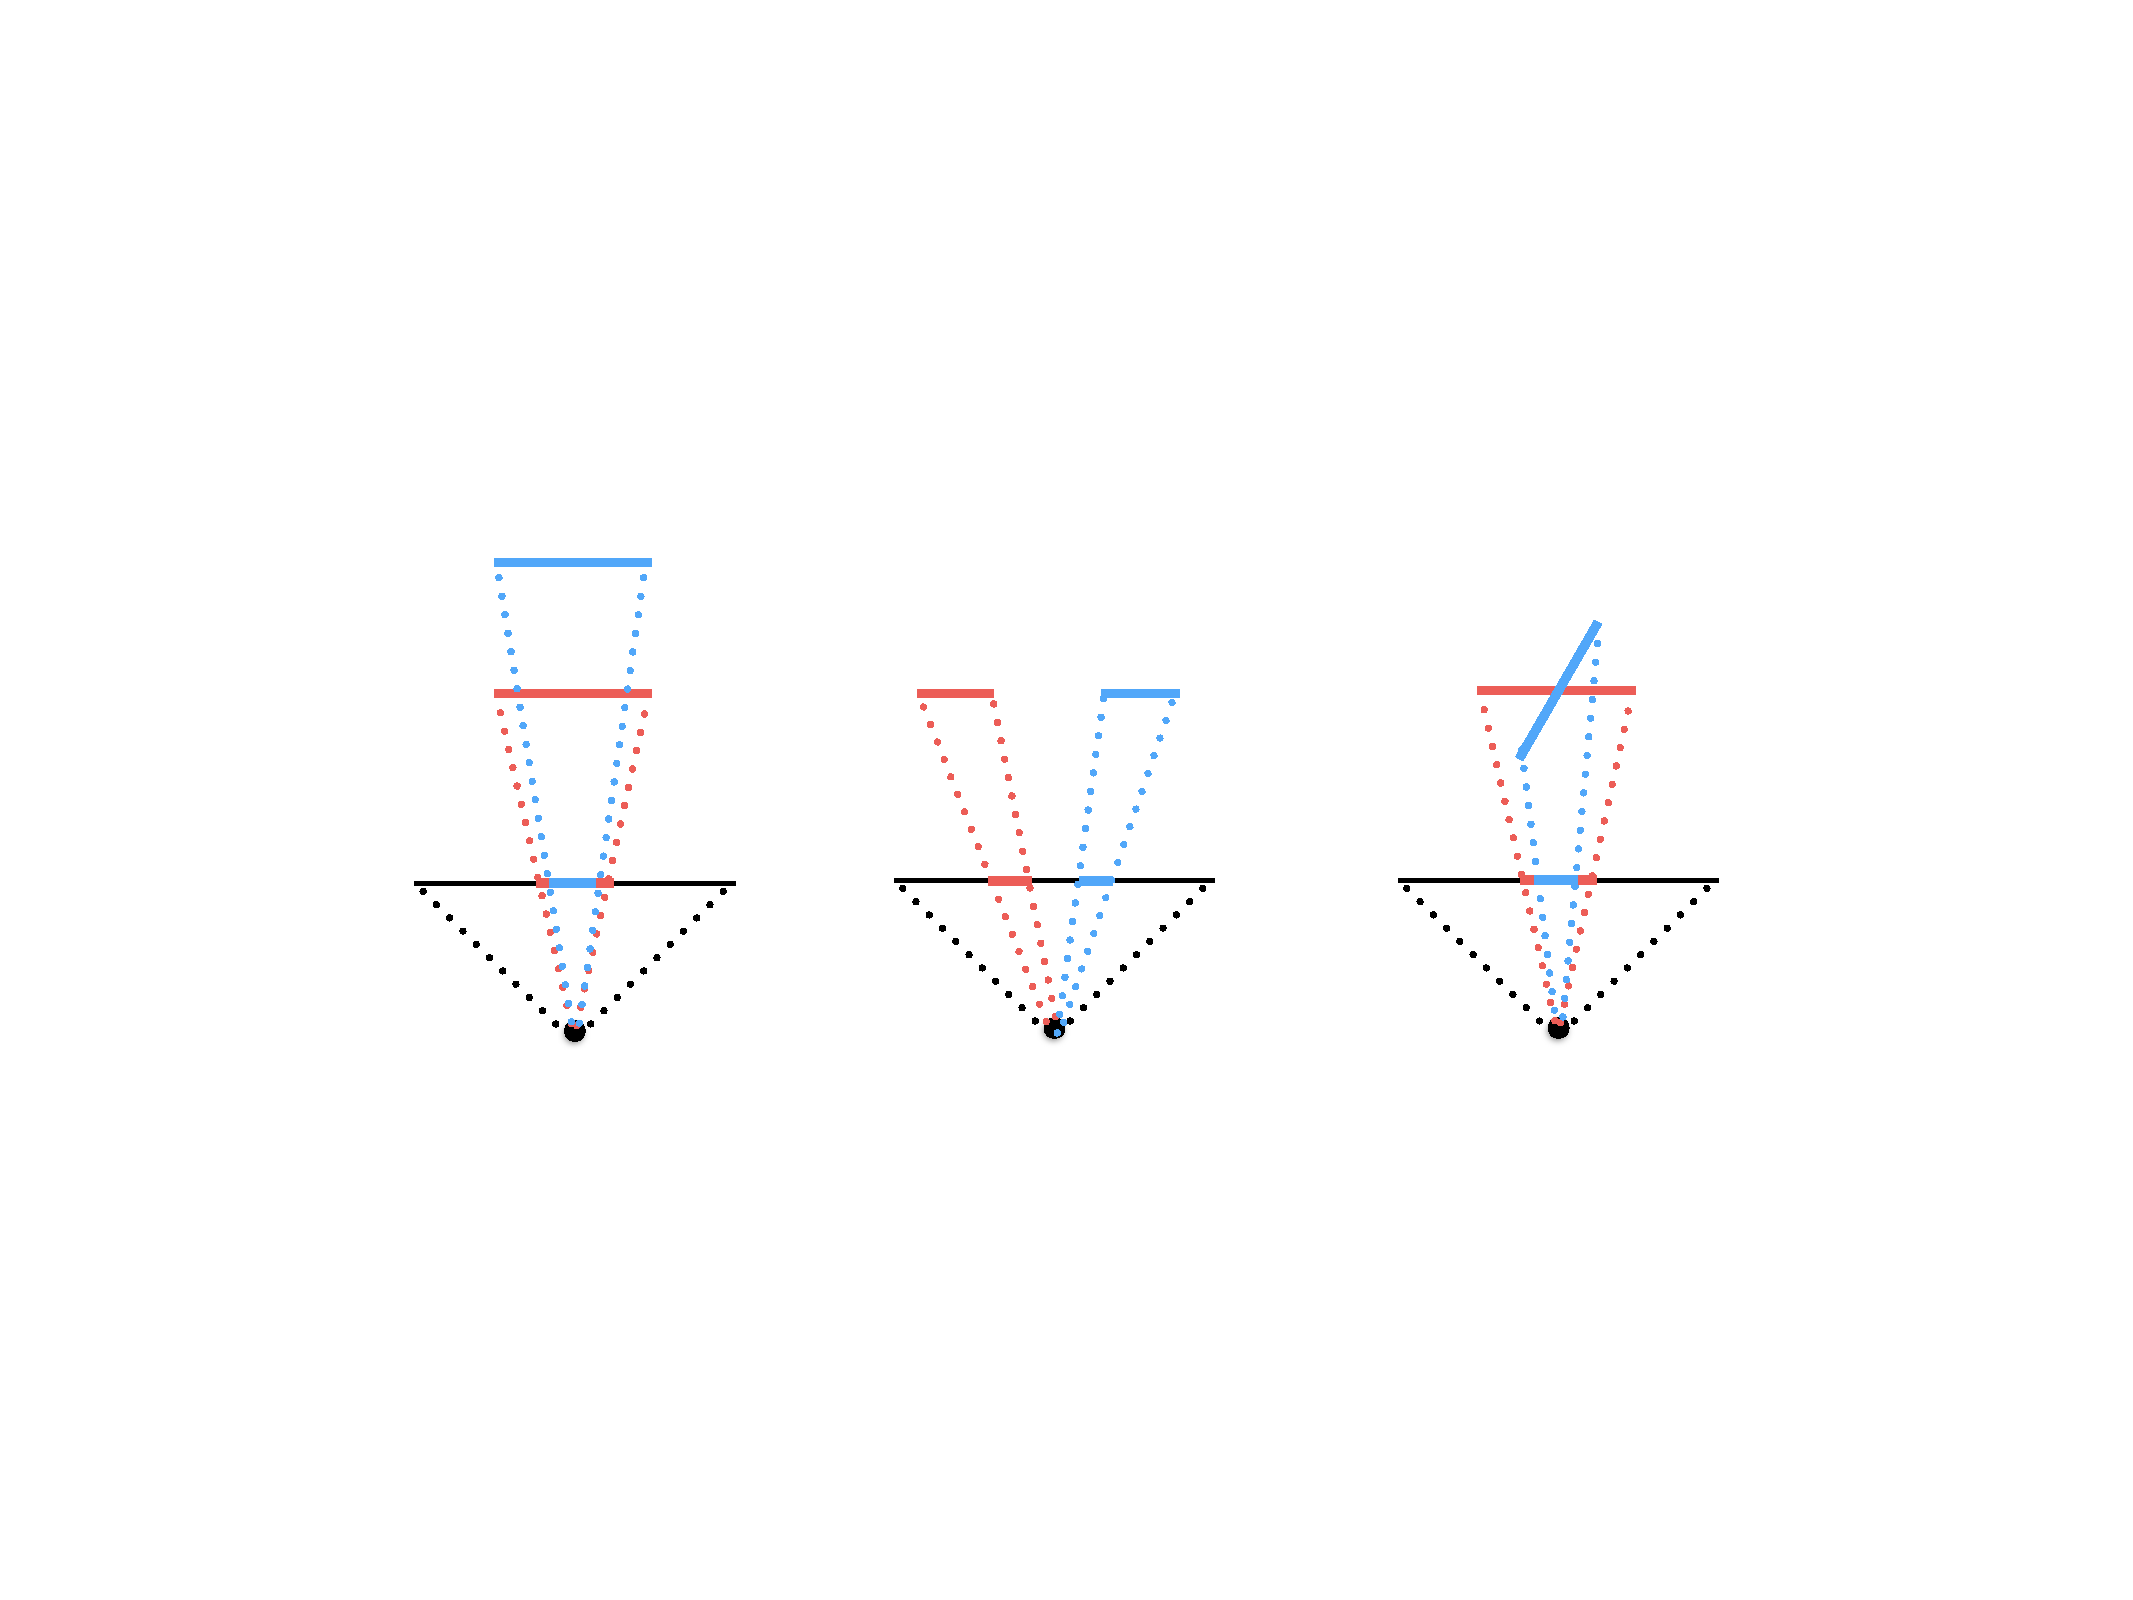
\includegraphics[width=0.8\textwidth]{relatedwork/tex_dist}
\caption{Three distortion effect: distance distortion, position distortion, and foreshortening distortion.}
\label{fig:tex_dist}
\end{figure}

To calculate the surface curvature at any point is far from trivial. Therefore, the surface shape is reconstructed by calculating the surface orientation (surface normal). A map of surface normals specifies the surface's orientation only at the points where the normals are computed. But, assuming that the normals are dense enough and the surface is smooth, the map can be used to reconstruct the surface shape.

\subsection{Defocus}
\textbf{Shape from focus}
A strong cue for object depth is the amount of blur, which increases as the object moves away from the camera's focusing distance. As shown in Figure~\ref{fig:thin_lens}, moving the object surface away from the focus plane increases the circle of confusion.

\begin{figure}[h]
\centering
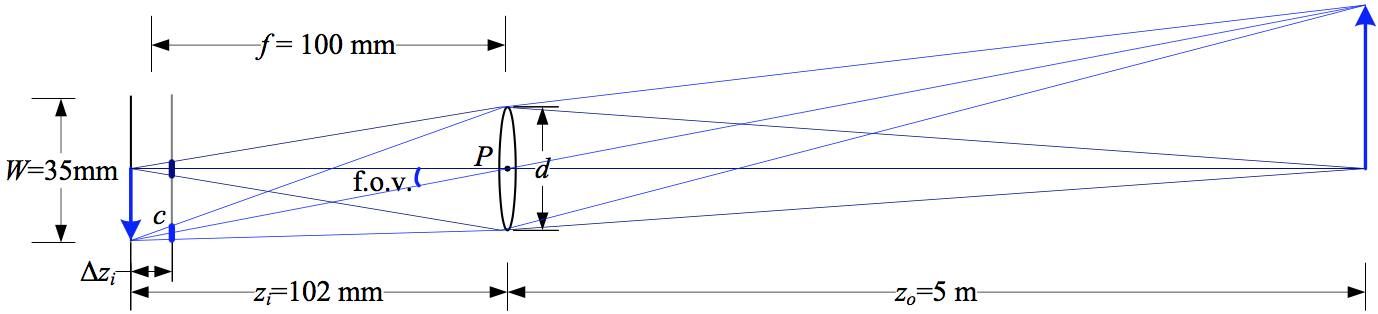
\includegraphics[width=0.8\textwidth]{relatedwork/thin_lens}
\caption{A thin lens of focal length $f$ focuses the light from a plane a distance $z_0$ in front of the lens at a distance $z_i$ behind the lens, where $\frac{1}{z_o}+\frac{1}{z_i}=\frac{1}{f}$. If the sensor plane moved forward $\Delta z_i$, the image are no longer in focus and the \textit{circle of confusion} $c$ depends on the distance of the sensor plane motion $\Delta z_i$ relative to the lens aperture diameter $d$.}
\label{fig:thin_lens}
\end{figure}

Figure~\ref{fig:thin_lens} shows the basic geometric image formation. The relationship between the object distance $z_o$, focal distance of the lens $f$, and the image distance $z_i$, is given by the Gaussian lens law:
$$
\frac{1}{z_o}+\frac{1}{z_i}=\frac{1}{f}
$$
All light rays that are radiated from the object and intercepted by the lens to converge at a single point on the image plane, thus a \textit{focused} image $I_f(x, y)$ is formed on the image plane. If, however, the sensor plane does not coincide with the image plane and is displaced from the image plane by a distance $\Delta z_i$, the energy received from the object is uniformly distributed over a circular patch on the sensor plane. The relationship between the radius $c$ of the circle of confusion and the sensor displacement $\Delta z_i$ is as follows:
$$
c = \frac{\Delta z_i r}{z_i}
$$
% where $r$ is the radius of the lens. If we assume that the radius $c$ of the circle of confusion is independent of the position of the object point. Therefore, the \textit{defocused} image $I_d(x, y)$ formed on the sensor plane can also be obtained by convolving the focused image $I_f(x, y)$ with a circular symmetric ``pillbox'' filter
% $$
% I_d(x, y)=p(x, y)*I_f(x, y)
% $$
% where
% $$
% p(x, y) = \begin{cases}
%     \frac{1}{\pi r^2}       & \quad \text{if } x^2+y^2\leq r^2\\
%     0  & \quad \text{otherwise}\\
%   \end{cases}
% $$
The defocused images can be obtained in three ways: by displacing the sensor with respect to the image plane, by moving the lens, or by moving the object with respect to the object plane. The first two ways cab cause the following problems:
\begin{itemize}
\item The magnification of the system varies, thereby causing the image coordinates of the object points to change.
\item The area on the sensor plane over which light energy is distributed varies, thereby causing a variation in image brightness.
\end{itemize}
To address this issue, the degree of focus is changed by moving the object with respect to a fixed configuration of the optical system and sensor. This approach ensures that the focused areas of the image are always subjected to the same magnification.

The idea is as follows: the stage is moved in increaments of $\Delta d$, and an image is captured at each stage position ($d=n\Delta d$). By studying the behaviour of the focus measure, an interpolation method is used to compute the accurate depth estimates from a small number of focus measures. An important feature of this method is the local nature, the depth estimate at an image point is computed only from focus measures recorded at that point.
\begin{figure}[h]
\centering
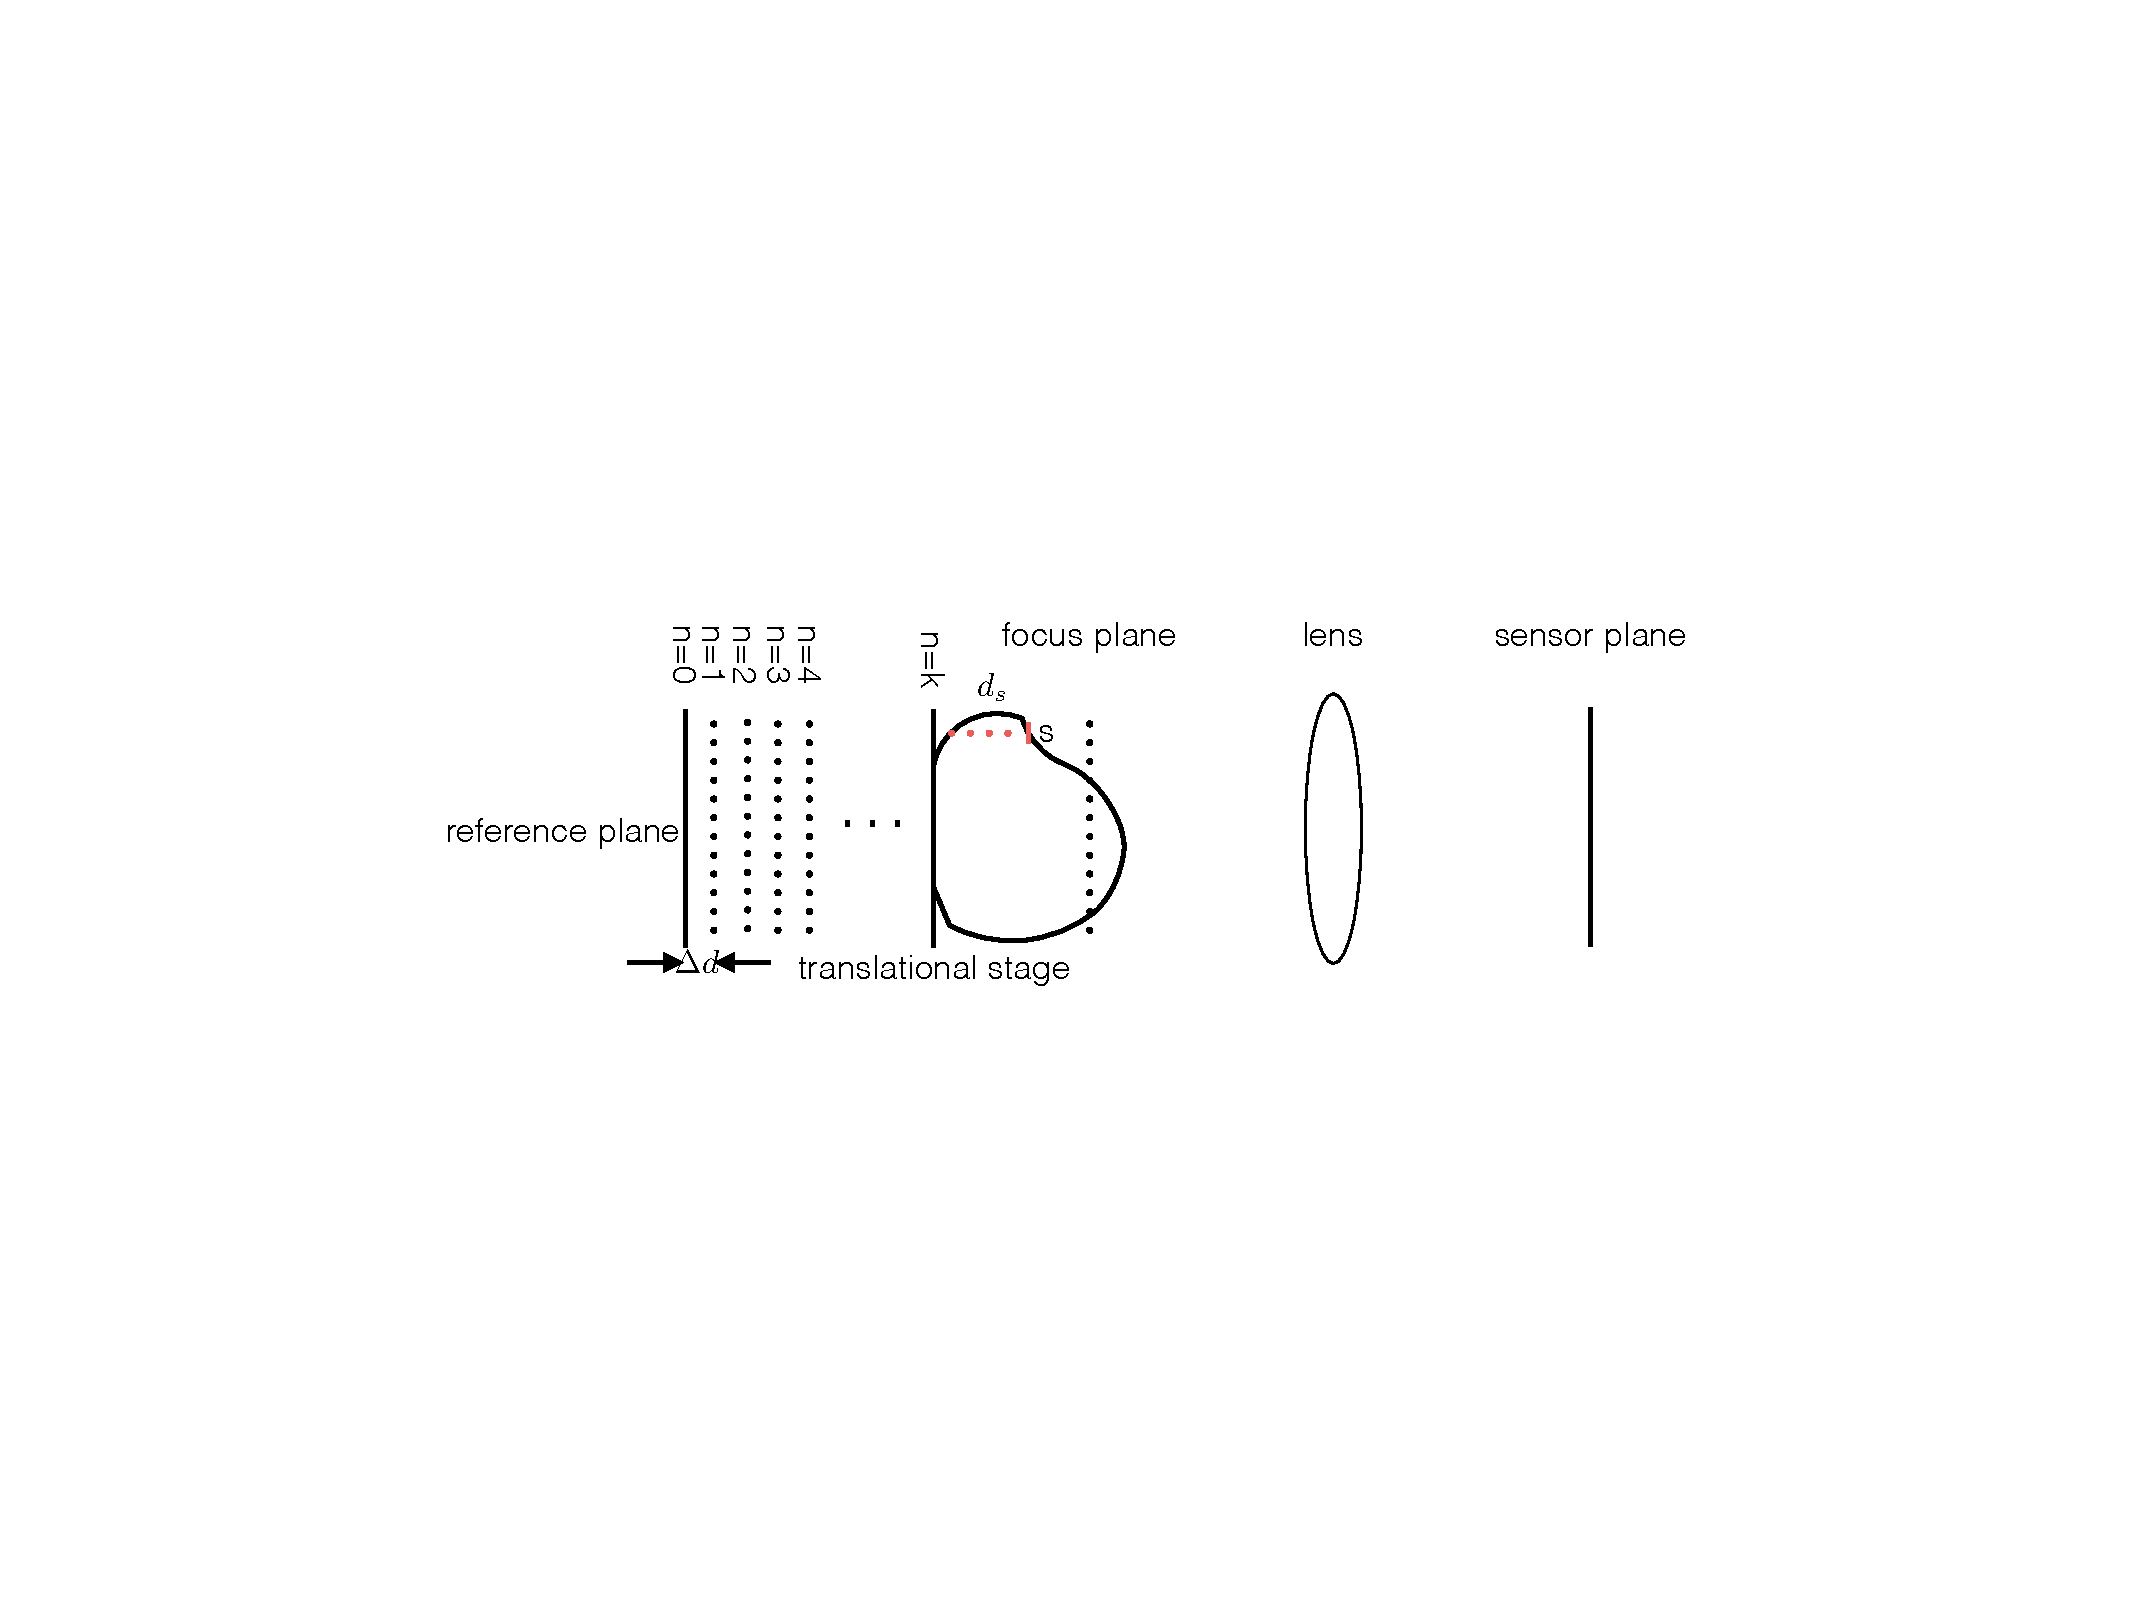
\includegraphics[width=0.8\textwidth]{relatedwork/shape_from_focus}
\caption{shape from focus}
\label{fig:shape_from_focus}
\end{figure}
